
\documentclass[12pt]{report}
\usepackage[a4paper]{geometry}
\usepackage[myheadings]{fullpage}
\usepackage{fancyhdr}
\usepackage{lastpage}
\usepackage{graphicx, wrapfig, subcaption, setspace, booktabs}
\usepackage[T1]{fontenc}
\usepackage[font=small, labelfont=bf]{caption}
\usepackage{fourier}
\usepackage[protrusion=true, expansion=true]{microtype}
\usepackage[english]{babel}
\usepackage{sectsty}
\usepackage{url, lipsum}
\usepackage{xcolor}
\usepackage{listings}
\usepackage{spverbatim}
\usepackage{hyperref}


\renewcommand{\thesection}{\arabic{section}}
\setcounter{section}{0} %numeracija sekcija

\graphicspath{ {./images/} }
\setlength\parindent{0pt} %nemoj uvuci paragraph
\newcommand{\code}[1]{\texttt{#1}} % code u tekstu

%color
\definecolor{my_green}{rgb}{0.027, 0.663, 0.545}
\newcommand{\mygreen}[1]{{\color{my_green}#1}}
\definecolor{my_red}{rgb}{0.843, 0.000, 0.384}
\newcommand{\myred}[1]{{\color{my_red}#1}}


%---- CODE LISTING
\definecolor{codecomment}{rgb}{0.561, 0.561, 0.561}
\definecolor{codegray}{rgb}{0.5,0.5,0.5}
\definecolor{codepurple}{rgb}{0.58,0,0.82}
\definecolor{pozadina}{rgb}{0.925, 0.925, 0.925,}


\lstdefinestyle{mystyle}{
    backgroundcolor=\color{pozadina},   
    commentstyle=\color{codecomment},
    keywordstyle=\color{magenta},
    numberstyle=\tiny\color{codegray},
    stringstyle=\color{codepurple},
	basicstyle=\ttfamily\footnotesize,
    breakatwhitespace=false,         
    breaklines=true,                 
    captionpos=b,                    
    keepspaces=true,                 
    numbers=left,                    
    numbersep=3pt,                  
    showspaces=false,                
    showstringspaces=false,
    showtabs=false,                  
    tabsize=2
}
\lstset{style=mystyle}
%--------



\begin{document}

\newcommand{\HRule}[1]{\rule{\linewidth}{#1}}
\onehalfspacing


%-------------------------------------------------------------------------------
% HEADER & FOOTER
%-------------------------------------------------------------------------------
\pagestyle{fancy}
\fancyhf{}
\setlength\headheight{15pt}
\fancyhead[L]{CANAL PLUS}


%-------------------------------------------------------------------------------
% FIRST PAGE
%-------------------------------------------------------------------------------
\title{ \normalsize \textsc{CANAL PLUS}
\\ [1.0cm]
\HRule{0.5pt} \\
\LARGE \textbf{\uppercase{TROUBLESHOOT ROOTFS}}
\HRule{2pt} \\ [0.5cm]
\normalsize  \vspace*{5\baselineskip}

\includegraphics[scale=0.8]{logo_rtrk.png}
}



\author{Miroslav Blazic}
\date{\today\\
    \fbox {Version: v1.0}
}

\maketitle


%-------------------------------------------------------------------------------
% TABLE OF CONTENT
%-------------------------------------------------------------------------------
\newpage
\tableofcontents
\newpage



\section*{ABSTRACT}
This document contains instruction of resolve infinite error during of setup NFS and ROOTFS for ali board.
Infinite error shown in the figure:
\begin{center}
    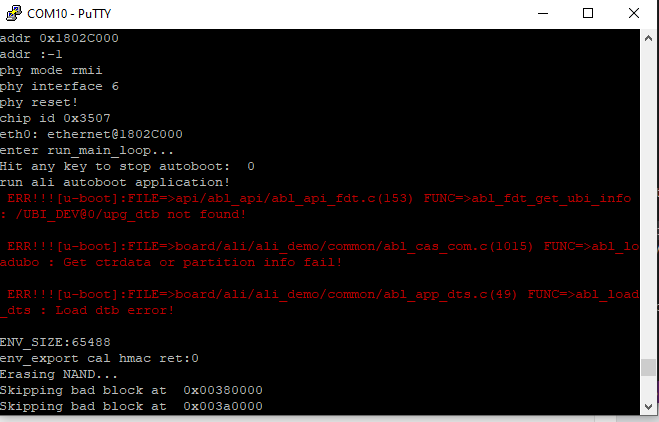
\includegraphics[scale=0.8]{error1.PNG}
\end{center}


\newpage


\section{INSTRUCTIONS OF TROUBLESHOOT}

An error occurs after burn process to ali board.
After we set up ROOTFS and NFS in \code{menuconfig} and \code{linux-menuconfig} we must not burn with select all modules.
We must burn with select only kernel.
When already occurs that error, unfortunately we can not solove to problem by just doing it burn with select only kernel, than we must to return to previous settings in \code{make menuconfig} and \code{make linux-menuconfig}.
Follow the next instructions in order to resolve that error.
\newline

Firstly, we need to set up configuration in the folowing way:
\newline
Menuconfig:\newline
- enable \code{squashfs root filesystem}\newline
- disable \code{nfs root filesystem} \newline
- disable \code{dhcp} \newline
\begin{lstlisting}[language=C]
    make menuconfig
\end{lstlisting}
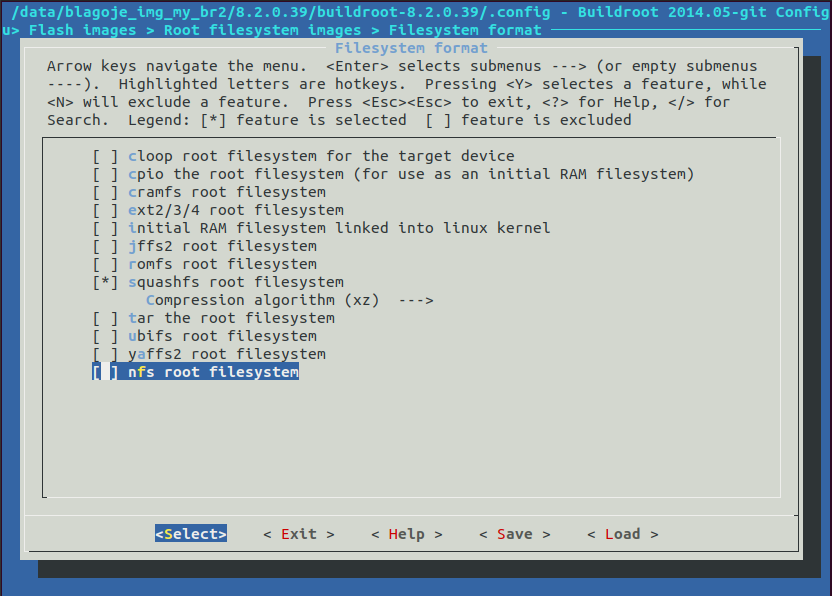
\includegraphics[scale=0.55]{1.PNG}
Save and exit.\newline

Linux-menuconfig:\newline
- disable \code{Root file system on NFS}
\begin{lstlisting}[language=C]
    make linux-menuconfig
\end{lstlisting}
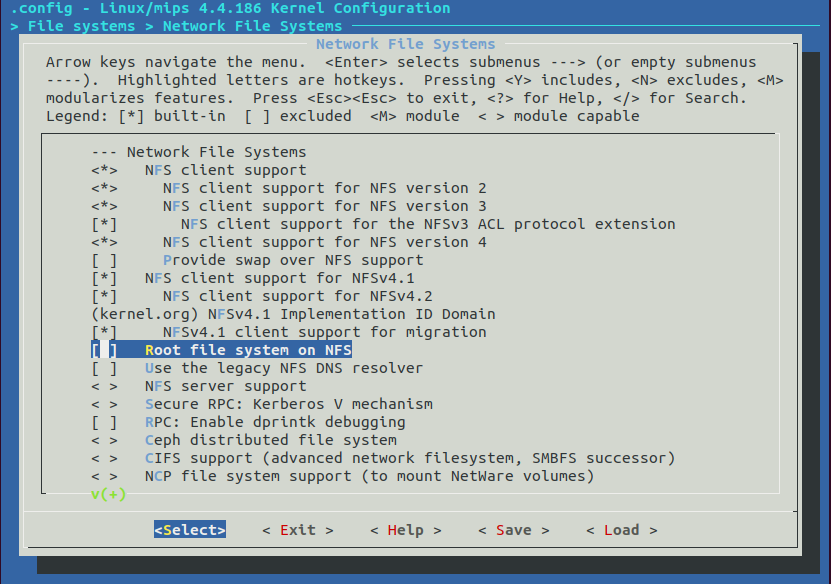
\includegraphics[scale=0.55]{2.PNG}
Save and exit. \newline

Run build process:
\begin{lstlisting}[language=C]
    make alim3538_ddk_c0200_nand_defconfig
    make dts-rebuild
    make linux-rebuild
    make all
\end{lstlisting}

With FT tool burn image (Select All modules) on board.\newline

Now we can set up configuration for NFS root filesystem:\newline
Menuconfig:\newline
- disable \code{squashfs root filesystem}\newline
- enable \code{nfs root filesystem} \newline
- enable \code{dhcp} \newline
\begin{lstlisting}[language=C]
    make menuconfig
\end{lstlisting}
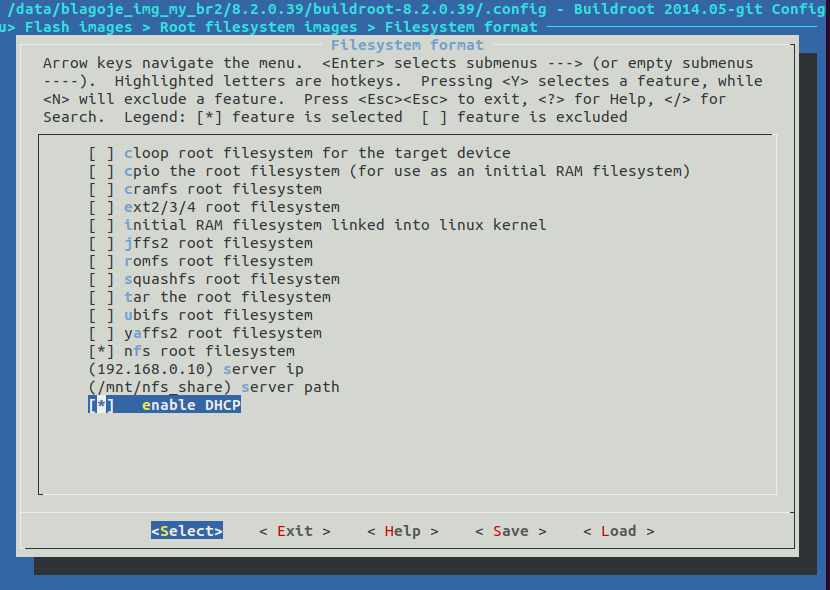
\includegraphics[scale=0.55]{3.PNG}
Save and exit.\newline

Linux-menuconfig:\newline
- enable \code{Root file system on NFS}
\begin{lstlisting}[language=C]
    make linux-menuconfig
\end{lstlisting}
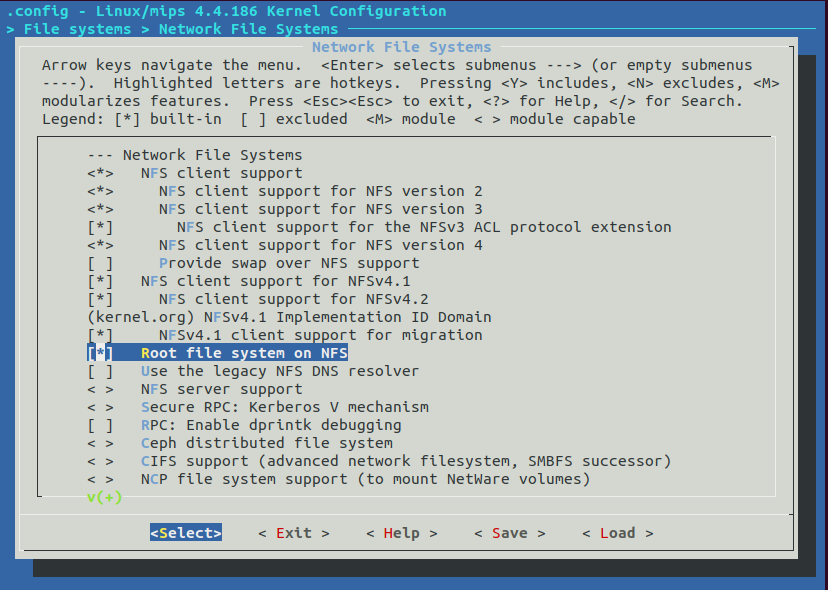
\includegraphics[scale=0.55]{4.PNG}
Save and exit.\newline

After complete configure \code{menuconfig} and \code{linux-menuconfig} you need to rebuild and burn with FT tool on ali board, but
this time burn only kernel! \newline
\begin{lstlisting}[language=C]
    make dts-rebuild
    make linux-rebuild
    make all
\end{lstlisting}
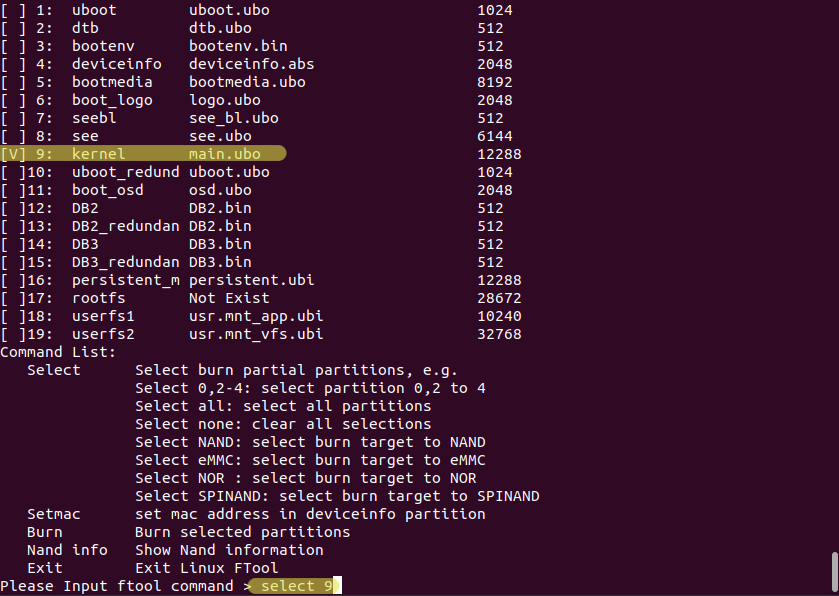
\includegraphics[scale=0.55]{5.PNG}




\end{document}